We conduct experiments with networks learnt on FashionMNIST~\cite{Xiao2017FashionMNIST}, and 22 binary labels of CelebA~\cite{liu2015faceattributes} datasets, Cat vs Dog (binary classification, 224x224x3 uncentered images),  and Imagenet~\cite{imagenet}. Note that labels in CelebA are very unbalanced (see~Table~2 in Appendix~A.2, with for instance less than $5\%$ samples for \textit{Mustache} or \textit{Wearing\_Hat}).% or \textit{Wearing\_Hat}). 

Architectures used for \otnn s~and unconstrained networks are similar (same number of layers and neurons, a VGG for FashionMNIST and CelebA, a ResNet50 for Cat vs Dog and Imagenet). We also train an alternative of ResNet50 OTNN with twice the number of parameters (50 M).  Unconstrained networks use batchnorm and ReLU layers for activation, whereas \otnn s~only use GroupSort2~\cite{pmlr-v97-anil19a,serrurier2021achieving} activation. \otnn s~are built using the \Deellip library, using Björck orthogonalization projection algorithm for linear layers. Note that several other approaches can be used for orthogonalization without altering the theoretical results; these might potentially enhance experimental outcome scores.
%*Loss
The loss functions are cross-entropy for unconstrained networks (categorical for multiclass, and sigmoid for multilabel settings), and hKR \losshkr~(and the multiclass variants see appendix A.2.3) for \otnn s. We train all networks with Adam optimizer~\cite{Diederik14Adam}. Details on architectures and parameters are given in Appendix~A.2.


\textbf{Classification performance:} \otnn~models achieve comparable results to  unconstrained ones, confirming claims of~\cite{bethunelip}: they reach 88.5\%
%\commentgreen{@Mathieu merci de remplir}
average accuracy on FashionMNIST
(Table~6), and 81\% (resp. 82\%) average Sensitivity (resp. Specificity) over labels on CelebA (Table~6 in Appendix~A.3). We use  Sensitivity and Specificity for CelebA to take into consideration the unbalanced labels. \otnn s~achieve 96\%  accuracy (98\% for the unconstrained version) on Cat vs Dog and 67\% (75\% for the unconstrained version) on Imagenet. The ResNet50 OTNN with 50M parameters achieves 70\% accuracy on Imagenet. 

%\subsection{Quantitative evaluation of explanations metrics}
% Please add the following required packages to your document preamble:
% \usepackage{multirow}
% \usepackage[table,xcdraw]{xcolor}
% If you use beamer only pass "xcolor=table" option, i.e. \documentclass[xcolor=table]{beamer}
\begin{table}[]
\begin{tabular}{lllllllll}
\cline{2-9}
\multicolumn{1}{c}{}                                     & \multicolumn{8}{c}{\cellcolor[HTML]{EFEFEF}\textbf{Dataset}}                                                                                                                                                                                   \\ \cline{2-9} 
\multicolumn{1}{c}{}                                     & \multicolumn{2}{c|}{Fash. MNIST}                                 & \multicolumn{2}{c|}{CelebA}                              & \multicolumn{2}{c|}{Cat vs Dog}                         & \multicolumn{2}{c}{Imagenet}                           \\
\multicolumn{1}{c}{\multirow{-3}{*}{}}                   & \multicolumn{1}{c|}{OTNN} & \multicolumn{1}{c|}{Uncst.}          & \multicolumn{1}{c|}{OTNN} & \multicolumn{1}{c|}{Uncst.}  & \multicolumn{1}{c|}{OTNN} & \multicolumn{1}{c|}{Uncst.} & \multicolumn{1}{c|}{OTNN} & \multicolumn{1}{c}{Uncst.} \\ \hline
\rowcolor[HTML]{EFEFEF} 
\multicolumn{1}{l|}{\cellcolor[HTML]{EFEFEF}Attribution} & \multicolumn{8}{c}{\cellcolor[HTML]{EFEFEF}\textbf{$\mu\text{Fidelity-Uniform}$ ($\uparrow$ is better)}}                                                                                                                                       \\ \hline
\multicolumn{1}{l|}{Saliency}                            & \textbf{0.156}            & \multicolumn{1}{l|}{-0.001}          & \textbf{0.244}            & \multicolumn{1}{l|}{0.052}   &                   \textbf{0.091}        & \multicolumn{1}{l|}{0.080}       &           \textbf{0.240 }          &  0.004                            \\
\multicolumn{1}{l|}{SmoothGrad}                          & \textbf{0.114}            & \multicolumn{1}{l|}{-0.001}          & \textbf{0.248}            & \multicolumn{1}{l|}{0.018}   &                  \textbf{0.012}         & \multicolumn{1}{l|}{-0.004}       &   \textbf{0.001}                         & -0.002                      \\
%\multicolumn{1}{l|}{Rise}                                & \textbf{0.220}            & \multicolumn{1}{l|}{0.011}           & \textbf{0.114}            & \multicolumn{1}{l|}{0.051}   &                  -0.002         & \multicolumn{1}{l|}{\textbf{0.014}}       &            \textbf{0.057}               &             -0.011                \\
\multicolumn{1}{l|}{Integ. Grad.}                                  & \textbf{-0.005}           & \multicolumn{1}{l|}{-0.013}          & \textbf{0.149}            & \multicolumn{1}{l|}{0.093}   &                   0.022        & \multicolumn{1}{l|}{\textbf{0.024}}       &          \textbf{0.046   }                     &        0.022                    \\
\multicolumn{1}{l|}{Grad. Input}                                  & -0.017                    & \multicolumn{1}{l|}{\textbf{-0.009}} & \textbf{0.168}            & \multicolumn{1}{l|}{0.074}   &                   \textbf{0.013}       & \multicolumn{1}{l|}{0.009}       &      \textbf{0.009 }        &           0.000                 \\
\multicolumn{1}{l|}{GradCam}                                  & \textbf{0.215}            & \multicolumn{1}{l|}{0.02}            & \textbf{0.028}            & \multicolumn{1}{l|}{0.002}   &                    \textbf{0.101}       & \multicolumn{1}{l|}{0.052}       &          0.029                 &               \textbf{0.046 }            \\ \hline
\rowcolor[HTML]{EFEFEF} 
\multicolumn{1}{l|}{\cellcolor[HTML]{EFEFEF}Attribution} & \multicolumn{8}{c}{\cellcolor[HTML]{EFEFEF}\textbf{$\mu\text{Fidelity-Zero}$  ($\uparrow$ is better)}}                                                                                                                                         \\ \hline
\multicolumn{1}{l|}{Saliency}                            & \textbf{0.246}            & \multicolumn{1}{l|}{0.034}           & \textbf{0.325}            & \multicolumn{1}{l|}{0.082}   & \textbf{0.121}            & \multicolumn{1}{l|}{0.079}  & \textbf{0.147}            & 0.049                      \\
\multicolumn{1}{l|}{SmoothGrad}                          & \textbf{0.332}            & \multicolumn{1}{l|}{0.052}           & \textbf{0.324}            & \multicolumn{1}{l|}{0.091}   & \textbf{0.011}            & \multicolumn{1}{l|}{-0.004} & 0.001                     & \textbf{0.002}             \\
%\multicolumn{1}{l|}{Rise}                                & \textbf{0.182}            & \multicolumn{1}{l|}{0.063}           & \textbf{0.350}            & \multicolumn{1}{l|}{0.190}   & \textbf{0.062}            & \multicolumn{1}{l|}{0.032}  & \textbf{0.023}            & 0.000                      \\
\multicolumn{1}{l|}{Integ. Grad.}                                  & \textbf{0.543}            & \multicolumn{1}{l|}{0.134}           & \textbf{0.400}            & \multicolumn{1}{l|}{0.125}   & \textbf{0.037}            & \multicolumn{1}{l|}{0.027}  & \textbf{0.057}            & 0.023                      \\
\multicolumn{1}{l|}{Grad. Input}                                  & \textbf{0.479}            & \multicolumn{1}{l|}{0.079}           & \textbf{0.439}            & \multicolumn{1}{l|}{0.093}   & \textbf{0.019}            & \multicolumn{1}{l|}{0.004}  & \textbf{0.020}            & -0.001                     \\
\multicolumn{1}{l|}{GradCam}                                  & \textbf{0.161}            & \multicolumn{1}{l|}{0.046}           & \textbf{0.127}            & \multicolumn{1}{l|}{0.061}   & \textbf{0.136}            & \multicolumn{1}{l|}{0.049}  & 0.048                     & \textbf{0.068}             \\ \hline
\rowcolor[HTML]{EFEFEF} 
\multicolumn{1}{c|}{\cellcolor[HTML]{EFEFEF}Attribution} & \multicolumn{8}{c}{\cellcolor[HTML]{EFEFEF}\textbf{Stability Spearman rank ($\downarrow$ is better)}}                                                                                                                                          \\ \hline
\multicolumn{1}{l|}{Saliency}                            & \textbf{0.59}             & \multicolumn{1}{l|}{0.91}            & \textbf{0.51}             & \multicolumn{1}{l|}{0.77}    &                    \textbf{0.58}      & \multicolumn{1}{l|}{0.69}       &\textbf{0.60 }                     &        0.74                    \\
\multicolumn{1}{l|}{SmoothGrad}                          & \textbf{0.55}             & \multicolumn{1}{l|}{0.82}            & \textbf{0.52}             & \multicolumn{1}{l|}{0.95}    &                \textbf{0.64}           & \multicolumn{1}{l|}{0.82}       &     \textbf{0.62}                    &          0.82               \\
\multicolumn{1}{l|}{Integ. Grad.}                                  & \textbf{0.61}             & \multicolumn{1}{l|}{0.79}            & \textbf{0.52}             & \multicolumn{1}{l|}{0.87}    &             \textbf{0.61}              & \multicolumn{1}{l|}{0.76}       &     \textbf{0.60 }                     &            0.74           \\ \hline
\rowcolor[HTML]{EFEFEF} 
\multicolumn{9}{c}{\cellcolor[HTML]{EFEFEF}\textbf{Distance Saliency smoothgrad ($\downarrow$ is better)}}                                                                                                                                                                                                \\ \hline
\multicolumn{1}{l|}{Saliency}                            & \textbf{7.5e-03}          & \multicolumn{1}{l|}{7.0e-02}         & \textbf{3.1e-4}          & \multicolumn{1}{l|}{1.4e-1} &          \textbf{3.7e-8 }                & \multicolumn{1}{l|}{4.1e-8}       &          \textbf{3.7e-8 }                &            4.3e-8                 \\ \hline
\rowcolor[HTML]{EFEFEF} 
%\multicolumn{9}{c}{\cellcolor[HTML]{EFEFEF}\textbf{Compression ($\downarrow$ is better)}}                                                                                                                                                                                                                 \\ \hline
%\multicolumn{1}{l|}{Saliency} &                           & \multicolumn{1}{l|}{}                                   & \textbf{9.5kb }                    & \multicolumn{1}{l|}{16.8kb}          &       \textbf{ 8.4kb}                   & \multicolumn{1}{l|}{8.9kb}       &            21.4kb             &       \textbf{20.9kb }                    \\ \hline
\end{tabular}
  \caption{Comparison of XAI metrics for different attributions methods and dataset for OTNN and unconstrained networks.}
\label{table:xaimetric}
\end{table}
We present the results of quantitative evaluations of XAI metrics to compare the Saliency Map method with other explanation methods on \otnn, and more generally compare XAI explanations methods on these networks and their unconstrained counterparts. On CelebA, we only present  the results for the label \textit{Mustache}, but results for the other labels are similar. Parameters for explanation methods and metrics are given in Appendix~A.4. We have chosen to present in Table \ref{table:xaimetric}  two SoTA XAI metrics that enable comparison between \otnn s~and unconstrained networks.  \textbf{$\mu\text{Fidelity}$ metric}~\cite{Bhatt20muFidelity} is a well-known method that measures the correlation between important variables defined by the explanation method and the model score decreases when these variables are reset to a baseline state (or replaced by uniform noise). Another important property for explanations is their stability for nearby samples. In~\cite{Yeh19InfidelityExplain}, the authors proposed Stability metrics based on the $L_2$ distance. To better evaluate this stability and make it comparable for different models, we replace the $L_2$ distance by $1-\rho$, $\rho$ being the Spearman rank correlation. Other model-dependent metrics are described in the Appendix. Results from the 50M parameter ResNet \otnn~are included in the human alignment study (Fig~\ref{fig:human_alignement}) to illustrate that enhancing the model's complexity can bolster both the accuracy and alignment. The following observations can be drawn from Table \ref{table:xaimetric}:
\iffalse
\subsubsection{Saliency Maps on \otnn~become reliable explanations}
\commentgreen{on s'etait fait critiqué sur des termes comme trusworrthy et reliable je pense qu'il faudrait changer ce titre de section: tentatives: \\
Enhanced scores for OTNNs Saliency Maps\\
%Good properties of OTNNs saleicy maps
\\
....
Ok vu tu supprime tout ca vu qu'il n'y a plus la tablleau
}
\fi

%\textbf{Insertion and Deletion metrics:} We first assess the quality of  Saliency Map explanations for the proposed network using Insertion and Deletion metrics~\cite{petsiuk18Rise}. Classical explanation methods, including the Saliency Map, are evaluated on CelebA and FashionMNIST datasets for both types of networks. Even if the score values cannot be compared between different networks, Table~\ref{tab:ins_del_metric} shows the Saliency Map method becomes competitive on these metrics and matches the top-ranking methods, whereas it is not the case for unconstrained networks. In Annex~\ref{ann:explanation_metrics}, we show that it is also the case for other metrics such as Robustness-SR~\cite{HsiehYLRKKH21}.

%\commentgreen{la parie deletion-insertion 0 c'est vraiment pas clair je pense qu'il faut l'enlever. On peut remplacer par robustnessSR si on arrive a faire FashionMNIST}.

% \iffalse
% \fel{Proposition: j'ai corrigé quelques typos dans la table et essayé de séparer des parties. Je ne suis pas sur que ce soit mieux, je laisse les deux et vous choisirez ;)}
% \begin{table}
%   \caption{Insertion and Deletion metrics evaluation; GC: GradCam, GI: Gradient.Input, IG: Integrated Gradient, Saliency Rk : Rank}
%   \label{tab:ins_del_metric_2}
%   \centering
%   \begin{tabular}{lc|cccccc}
%     \toprule
% Dataset& Network&  \multicolumn{6}{c}{Deletion-Uniform (lower is better)}  \\
% & & GC & GI & IG & Rise& Saliency& SmoothGrad\\
%  \midrule
% CelebA& \otnn & 9.41& 9.38& 9.36& 8.89& 8.32 (Rk2) & \textbf{8.28}\\
% & Unconstrained& 5.13& 3.33& \textbf{3.18}& 3.61& 3.50 (Rk4) & 3.41\\
% Fashion-& \otnn& 0.23& 0.28& 0.28& 0.24& 0.22 (Rk2) & \textbf{0.21}\\
% MNIST & Unconstrained& 0.32& 0.35& 0.39& 0.32& 0.26 (Rk2) & \textbf{0.24}\\
%  \midrule
% & &  \multicolumn{6}{c}{Insertion Uniform (higher is better)} \\
% CelebA& \otnn& 10.25& 10.44& 10.50& 10.46& \textbf{11.29} (Rk1) & 11.28\\
% & Unconstrained& 9.43& 8.45& 9.24& \textbf{12.20} & 6.71 (Rk6) & 6.72\\
% Fashion-& \otnn& \textbf{0.28}& 0.20& 0.20& 0.26& 0.25 (Rk4) & 0.26\\
% MNIST & Unconstrained& \textbf{0.44} & 0.32& 0.26& 0.40& 0.30 (Rk4)& 0.24\\
%     \bottomrule
%     \end{tabular}
% \end{table}
% \fi 



\textbf{Saliency Map on \otnn s exhibit more fidelity and stability : } 
We confirm and amplify the results in ~\cite{felHowGood22}. Table.~\ref{table:xaimetric} clearly states that 
%Table.~\ref{table:xaimetric} confirms and amplifies the results in ~\cite{felHowGood22}, clearly stating that 
for most of the explanation methods, the $\mu\text{Fidelity}$,  zero or uniform, is significantly higher for \otnn s. And above all, Saliency Map score for \otnn s~is always higher than any other attribution method score for unconstrained models.
%whatever the explanation method, the $\mu\text{Fidelity}$, with zero or uniform score modification, is significantly higher when it is applied on \otnn. There are instances where this is not the case for the ResNet architecture; however, in such cases, the Saliency Map of OTNN significantly outperforms any attribution metrics for unconstrained models. 
%This confirms and amplify the result ~\cite{felHowGood22}, which shows that \onlyonelip~ neural networks, for the two proposed metrics, produce explanations with higher scores than common neural networks (\mathieu{A améliorer}). 
A similar observation 
holds for 
%applies to 
the Stability Spearman rank
: \otnn~scores are better whatever the attribution method.
%, where the score is substantially better for \otnn, regardless the attribution considered.


\textbf{Saliency Map method on \otnn s~is equivalent to other attribution methods: }
We observe that the scores from the Saliency Maps and other methods are very similar for \otnn, with Saliency Maps consistently ranking among the top attribution methods. For the unconstrained case, Saliency Maps are occasionally outperformed by other attribution methods. Notably, for the ResNet architecture, attribution methods other than Saliency Maps and GradCAM yield more erratic results for fidelity metrics. To highlight these results, we compare the $L_2$ distance between Saliency Maps and SmoothGrad explanations, as suggested by \cite{Adebayo18Sanity,felHowGood22,tomsett2019sanity,ghorbani2017interpretation}. The explanation distances for \otnn~are significantly lower than for the unconstrained ones and closely approach zero, indicating that for \otnn, averaging over a large set of noisy inputs—as in SmoothGrad—is unnecessary. This is illustrated in Fig.\ref{fig:saliency_smoothgrad}.
\iftrue
\begin{figure*}
\begin{tabular}{@{}c@{}cc@{}}
\centering
    \begin{tabular}{c}
  \rowcolor{white}  \rotatebox{90}{\textbf{Saliency}}
  \end{tabular} & 
  \begin{tabular}{@{}l@{}l@{}l@{}}
    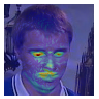
\includegraphics[width=.16\linewidth]{img/saliency_smoothgrad/saliency_1Lip_3_crop.png} &
  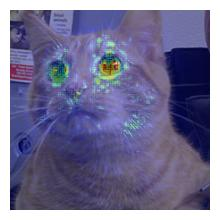
\includegraphics[width=.16\linewidth]{img/catvsdog/OTNN_saliency_1.jpg} & 
  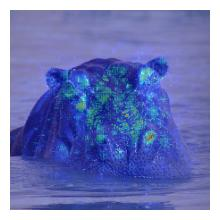
\includegraphics[width=.16\linewidth]{img/imagenet/OTNN_saliency_2.jpg}
  \end{tabular} & 
  \begin{tabular}{@{}l@{}l@{}l@{}}
  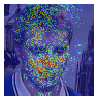
\includegraphics[width=.16\linewidth]{img/saliency_smoothgrad/saliency_Unconst_3_crop.png} &
  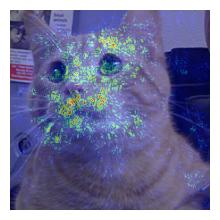
\includegraphics[width=.16\linewidth]{img/catvsdog/resnet50_saliency_1.jpg} & 
  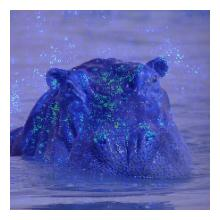
\includegraphics[width=.16\linewidth]{img/imagenet/resnet50_saliency_2.jpg}
  \end{tabular}\\

  \begin{tabular}{l}
   \rotatebox{90}{\textbf{SmoothGrad}} 
  \end{tabular} &
  \begin{tabular}{@{}l@{}l@{}l@{}} 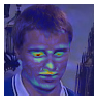
\includegraphics[width=.15\linewidth]{img/saliency_smoothgrad/smoothgrad_1Lip_3_crop.png} &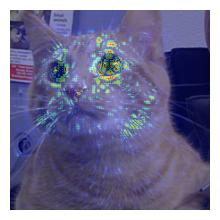
\includegraphics[width=.16\linewidth]{img/catvsdog/OTNN_smooth_1.jpg} & 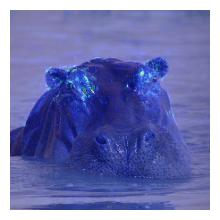
\includegraphics[width=.16\linewidth]{img/imagenet/OTNN_smooth_2.jpg}
  \end{tabular} & 
  \begin{tabular}{@{}l@{}l@{}l@{}}
  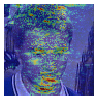
\includegraphics[width=.16\linewidth]{img/saliency_smoothgrad/smoothgrad_Unconst_3_crop.png} & 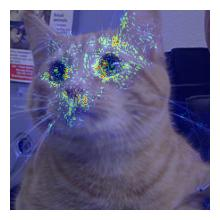
\includegraphics[width=.16\linewidth]{img/catvsdog/resnet50_smooth_1.jpg} & 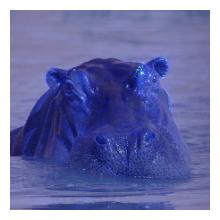
\includegraphics[width=.16\linewidth]{img/imagenet/resnet50_smooth_2.jpg}
  \end{tabular}\\
& (a)~\otnn
  &  (b) Unconstrained
\end{tabular}
\caption{Comparison of Saliency Map and SmoothGrad  explanations for (a) \otnn~ and (b) unconstrained network for, from left to right, CelebA, Cat vs Dog and Imagenet datasets.} %\commentgreen{Thomas a donné des nouvelles images elles sont dans saliency_smoothgrad/robust... a mettre en annexe ou ici }}
\label{fig:saliency_smoothgrad}
\end{figure*}
\fi

\iffalse
\begin{figure*}
\begin{tabular}{@{}c@{}c@{}c}
\centering
  \begin{tabular}{l}
    \rotatebox{90}{\textbf{Saliency}}
  \end{tabular}
 & 
  \begin{tabular}{@{}l@{}l@{}l}
    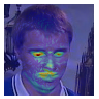
\includegraphics[width=.14\linewidth]{img/saliency_smoothgrad/saliency_1Lip_3_crop.png} &
  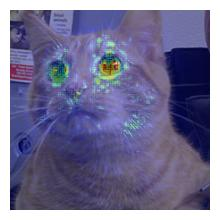
\includegraphics[width=.15\linewidth]{img/catvsdog/OTNN_saliency_1.jpg} %& 
%  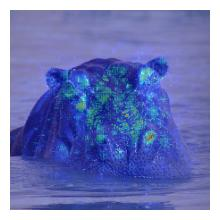
\includegraphics[width=.15\linewidth]{img/imagenet/OTNN_saliency_2.jpg}
  \end{tabular} &
  \multirow{6}{c}{\includegraphics[width=.35\textwidth]{img/human_alignment.jpg}}
  \\

  \begin{tabular}{l}
   \rotatebox{90}{\textbf{SmoothGrad}} 
  \end{tabular} &
  \begin{tabular}{@{}l@{}l@{}l} 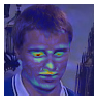
\includegraphics[width=.14\linewidth]{img/saliency_smoothgrad/smoothgrad_1Lip_3_crop.png} &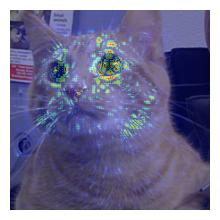
\includegraphics[width=.15\linewidth]{img/catvsdog/OTNN_smooth_1.jpg} %& 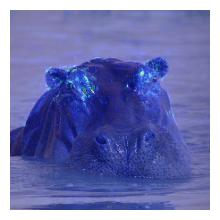
\includegraphics[width=.15\linewidth]{img/imagenet/OTNN_smooth_2.jpg}
  \end{tabular} &  \\
& (a)~\otnn  & \\
  \begin{tabular}{l}
    \rotatebox{90}{\textbf{Saliency}}
  \end{tabular}
 & 
  \begin{tabular}{@{}l@{}l@{}l}
  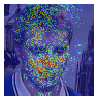
\includegraphics[width=.15\linewidth]{img/saliency_smoothgrad/saliency_Unconst_3_crop.png} &
  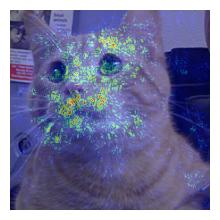
\includegraphics[width=.16\linewidth]{img/catvsdog/resnet50_saliency_1.jpg} %& 
%  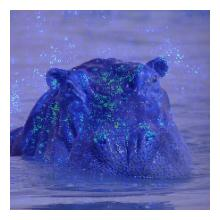
\includegraphics[width=.15\linewidth]{img/imagenet/resnet50_saliency_2.jpg}
  \end{tabular}  & \\
  \begin{tabular}{l}
   \rotatebox{90}{\textbf{SmoothGrad}} 
  \end{tabular} &
  \begin{tabular}{@{}l@{}l@{}l}
  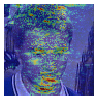
\includegraphics[width=.15\linewidth]{img/saliency_smoothgrad/smoothgrad_Unconst_3_crop.png} & 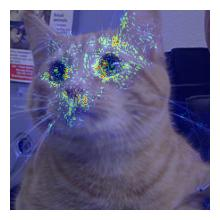
\includegraphics[width=.16\linewidth]{img/catvsdog/resnet50_smooth_1.jpg} %& 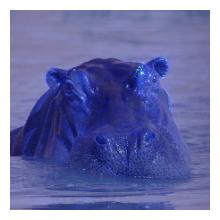
\includegraphics[width=.15\linewidth]{img/imagenet/resnet50_smooth_2.jpg}
  \end{tabular} & \\
&   (b) Unconstrained& 
\end{tabular}
\caption{Comparison of Saliency Map and SmoothGrad  explanations for (a) \otnn~ and (b) unconstrained network for the respectively CelebA, cat vs dog and imagenet.} %\commentgreen{Thomas a donné des nouvelles images elles sont dans saliency_smoothgrad/robust... a mettre en annexe ou ici }}
\label{fig:saliency_smoothgrad}
\end{figure*}
\fi
%\textbf{Saliency Map on \otnn~are less complex:} 
%Complexity of a given explanation is linked to the understandability by a human. \commentgreen{Thomas si tu as des references ? TBC should be kolmogorov but JPEG is a good surrogate}
%Inspired by previous works~\cite{da2011image} highlighting a strong correlation between Kolmogorov complexity and human evaluation of complexity~\cite{forsythe2008confounds,forsythe2009visual}. We used a JPEG based compressor~\cite{vereshchagin2005lossy} as a simple approximation of  visual explanation complexity~\cite{li2004similarity}: \otnn s~yield simpler explanations than unconstrained networks in all case. %($16.8kB$) -see Figure~\ref{fig:saliency_smoothgrad} for a qualitative comparison-.
%. \commentgreen{il manque les resultats (a faire Franck)}



%\subsubsection{\otnn s~ provide better explanations}
%\commentgreen{idem better ca veut pas dire grand chose\\
%\otnn s~ explanations exhibit more fidelity and stability\\
%...\\
%d'autres propositions?}





\textbf{\otnn s~ explanations are aligned with human ones : }
Adopting the method presented in~\cite{linsley2017visual}, using the ClickMe dataset, we follow strictly their experimental methodology and use their code\footnote{https://github.com/serre-lab/Harmonization} to compute the human feature alignment of OTNN Saliency Maps and compare with the others models tested in ~\cite{ fel2022aligning}-- more than 100 recent deep neural networks. In Figure ~\ref{fig:human_alignement}, we demonstrate that 
OTNN models Saliency Maps, %the Saliency Map of  the OTNN model,
which also carries a theoretical interpretation as the direction of the transport plan,  is more aligned with human attention than any other tested models and significantly surpasses the Pareto front discovered by~\cite{fel2022aligning}. The OTNN model is even more aligned than a ResNet50 model trained with a specific alignment objective, proposed by~\cite{fel2022aligning}, and called \textit{Harmonized ResNet50}. 
This finding is interesting as it indicates \otnn s are less prone to relying on spurious correlations~\cite{geirhos2020shortcut} and 
%is more adept at capturing 
better capture
human visual strategies for object recognition.
%The implications of these findings are crucial first for cognitive science: A model with closer alignment with human attention and visual strategies can provide a more comprehensive understanding of how vision operates for humans. Besides, it enhances the predictability, interpretability, and performance of object recognition models which as positive consequences in industry settings.
The implications of these results are crucial for both cognitive science and industrial applications. A model that more closely aligns with human attention and visual strategies can provide a more comprehensive understanding of how vision operates for humans, and also enhance the predictability, interpretability, and performance of object recognition models in industry settings. 
Furthermore, the drop in alignment observed in recent models highlights the necessity of considering the alignment of model visual strategies with human attention while developing object recognition models to reduce the reliance on spurious correlations and ensure that our models get things right for the right reasons.

\iftrue
\begin{figure*}
\centering
\includegraphics[width=1.\textwidth]{img/human_alignment_flat_2.pdf}
\caption{\textbf{\otnn~are aligned with Human attention.} Our study shows that the Saliency Map of OTNN model is highly aligned with human attention.% This finding is supported by the work of~\cite{fel2022aligning}, which demonstrates the trade-off between deep neural network (DNN) performance and alignment with human feature importance from the ClickMe~\cite{linsley2017visual} dataset. The degree of alignment between human and DNN saliency is measured using the mean Spearman correlation, normalized by the average inter-rater alignment of humans. 
%Among the hundreds of model tests performed in the original study, our model is the only one that breaks the Pareto front, suggesting a superior trade-off between DNN performance and alignment with human attention. Even an Harmonized model from~\cite{fel2022aligning} study, which was specifically designed to predict human attention, achieves a lower alignment than our model. \fel{on peut remove ca si vous voulez:} Overall, our results highlight the potential of the OTNN model to capture the visual strategies used by humans for object recognition, and may lead to improved performance and interpretability of object recognition models in both cognitive science and industry applications.
}
\label{fig:human_alignement}
\end{figure*}
\fi



\iffalse
\begin{figure*}
\centering
\includegraphics[width=.7\textwidth]{img/human_alignment.jpg}
\caption{\textbf{\otnn~are aligned with Human attention.} Our study shows that the Saliency Map of \otnn~model is highly aligned with human attention.% This finding is supported by the work of~\cite{fel2022aligning}, which demonstrates the trade-off between deep neural network (DNN) performance and alignment with human feature importance from the ClickMe~\cite{linsley2017visual} dataset. The degree of alignment between human and DNN saliency is measured using the mean Spearman correlation, normalized by the average inter-rater alignment of humans. 
%Among the hundreds of model tests performed in the original study, our model is the only one that breaks the Pareto front, suggesting a superior trade-off between DNN performance and alignment with human attention. Even an Harmonized model from~\cite{fel2022aligning} study, which was specifically designed to predict human attention, achieves a lower alignment than our model. \fel{on peut remove ca si vous voulez:} Overall, our results highlight the potential of the OTNN model to capture the visual strategies used by humans for object recognition, and may lead to improved performance and interpretability of object recognition models in both cognitive science and industry applications.
}
\label{fig:human_alignement}
\end{figure*}
\fi
%Reseau normal: Grad => metriques nulles; comparer avec autre methode d'explication
%Reseau hKR: Grad => metriques++; eventuellement comparer autres explications 
%Metriques: robustnes-Sr; stability; .... (voir avec thomas les autres potentiellement deja dans xplique qu'on pourrait tester )
%\subsection{adult} explaination show unfairness

%\subsection{Qualitative results}
\textbf{Qualitative results: }
Using the learnt \otnn~on FashionMNIST, CelebA (Mouth Slightly Open label), Cat vs Dog and Imagenet, Fig.~\ref{fig:celebA_counterfactual},\ref{fig:fashionMNIST_counterfactual}  present the original image, average gradients $\nabla_x f_j$  over the channels, and images in the direction of the transport plan (Prop.~\ref{th:gradient_transport_plan}), other samples are given in Appendix~A.5. 
We can see that most of the gradients are visually consistent, showing clearly what has to be changed in the input image to modify the class and act as a counterfactual explanation. 
%what needed to change in the input image to classes and act as a counterfactual explanation. 
This is less clear for the Imagenet examples. This could be due to the difficulty of defining a transport plan for each pair of the 1000 classes. However, feature visualizations in Figure \ref{fig:big_picture} show that the internal representation of the classes is still more interpretable than the unconstraint one. 
More generally, we observe that the gradient gives clear information about how the classifier makes its decision. For instance, for the cat, it shows that the classifier does not need to encode perfectly the concept of a cat, but mainly to identify the color of the eyes and size of the nose.
%\commentgreen{@Mathieu tu en feras d'autres images sinon enlever la paranthese}

\iffalse
\begin{figure*}
    \centering
        \begin{tabular}{ccc}
        \multicolumn{3}{c}{CelebA Mouth Slightly Open label: left close to open, right open to close} \\
        \begin{tabular}{ccc}
            \includegraphics[width=.13\linewidth]{img/Mouth_slightly_open/00024_input_lbl0_fx-0.59.pdf} & \includegraphics[width=.13\linewidth]{img/Mouth_slightly_open/00024_gradColor.pdf} & \includegraphics[width=.13\linewidth]{img/Mouth_slightly_open/00024_xMinus10.0Grad.pdf} 
        \end{tabular} &
        \begin{tabular}{ccc}
            \includegraphics[width=.13\linewidth]{img/Mouth_slightly_open/00072_input_lbl1_fx0.47.pdf} & \includegraphics[width=.13\linewidth]{img/Mouth_slightly_open/00072_gradColor.pdf} & \includegraphics[width=.13\linewidth]{img/Mouth_slightly_open/00072_xMinus10.0Grad.pdf} 
        \end{tabular} & \\
         %\midrule
          
        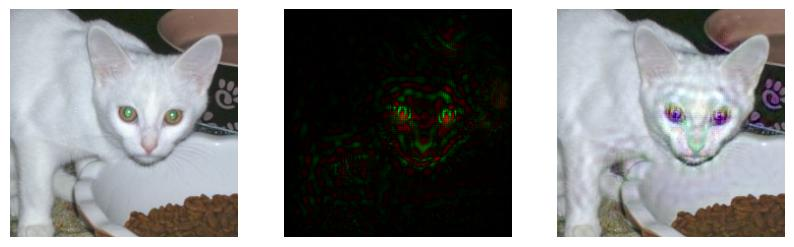
\includegraphics[width=.5\linewidth] {img/catvsdog/expl_1.jpg} &
        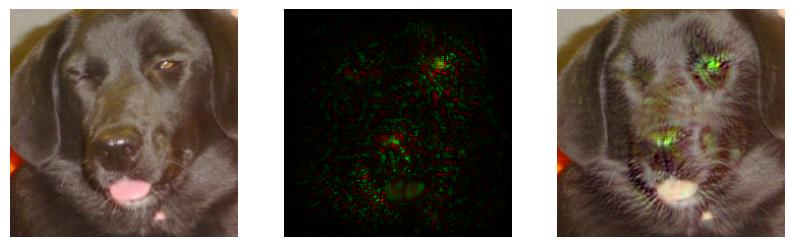
\includegraphics[width=.5\linewidth] {img/catvsdog/expl_2.jpg} & \\
        % \midrule
        \multicolumn{3}{c}{Imagenet :left cabbage butterfly to monarch one,  right great grey owl to bald eagle} \\
        
\includegraphics[width=.5\linewidth] {img/imagenet/expl_1.jpg} &
        
\includegraphics[width=.5\linewidth] {img/imagenet/expl_2.jpg} %\\
        & \\
     \end{tabular}
    \caption{Samples of conterfactuals from different dataset: (left) source image , (center) gradient image, (right) counterfactual of the form $\x-t*\hat{f}(\x)\nabla_x \hat{f}(\x)$, for  $t>1$}
    \label{fig:celebA_counterfactual}
\end{figure*}


\begin{figure*}[h]
  \centering
  \fbox{\includegraphics[width=0.98\linewidth]{img/fashion-otnn.png}}
  
\caption{Samples from different classes of FashionMNIST: (left) source image , (center) targeted gradient image of an \otnn, (right) targeted counterfactual of the form $\x-10*\hat{f}(\x)\nabla_x \hat{f}(\x)$}
%Counterfactuals of the form $ \x-10*\hat{f}(\x)\nabla_x \hat{f}(\x)$  of a \otnn~ for FashionMNIST. }
\label{fig:fashion_mnist}
\end{figure*}
\fi


\begin{figure*}
\centering
\begin{tabular}{ccc}
%\multicolumn{3}{c}{Fashion MNIST source image and class, targeted gradient image and counterfactual.} \\
\multicolumn{3}{c}{\includegraphics[width=1.0\linewidth]{img/fashion-otnn.pdf}}\\
\end{tabular}
\caption{Samples of counterfactuals for FashionMNIST dataset on different classes and targets: (left) source image , (center) gradient image, (right) counterfactual of the form $\x-t*\hat{f}(\x)\nabla_x \hat{f}(\x)$, for  $t>1$}
\label{fig:fashionMNIST_counterfactual}
\end{figure*}

\iftrue
\begin{figure*}
    \centering
    \begin{tabular}{rcc}
        %\multicolumn{3}{c}{Fashion MNIST source image and class, targeted gradient image and counterfactual.} \\
        %\multicolumn{3}{c}{\includegraphics[width=1.0\linewidth]{img/fashion-otnn.pdf}}\\
        %\multicolumn{3}{c}{CelebA Mouth Slightly Open label: left close to open, right open to close} \\
        \rotatebox[origin=c]{90}{CelebA}\hspace{-5mm} & 
        \begin{tabular}{ccc}
            \includegraphics[width=.13\linewidth]{img/Mouth_slightly_open/00024_input_lbl0_fx-0.59.pdf} & \includegraphics[width=.13\linewidth]{img/Mouth_slightly_open/00024_gradColor.pdf} & \includegraphics[width=.13\linewidth]{img/Mouth_slightly_open/00024_xMinus10.0Grad.pdf}\\
            % \textbf{mouth closed} & $\to$ & \textbf{mouth opened}
        \end{tabular} &
        \begin{tabular}{ccc}
            \hspace{-4mm}
            \includegraphics[width=.13\linewidth]{img/Mouth_slightly_open/00072_input_lbl1_fx0.47.pdf} & \includegraphics[width=.13\linewidth]{img/Mouth_slightly_open/00072_gradColor.pdf} & \includegraphics[width=.13\linewidth]{img/Mouth_slightly_open/00072_xMinus10.0Grad.pdf} \\
            % \textbf{mouth opened} & $\to$ & \textbf{mouth closed}
        \end{tabular} \\
          & \textbf{mouth closed $\to$ mouth opened} &  \textbf{mouth opened $\to$ mouth closed}\\
        %\midrule
        % \multicolumn{3}{c}{CelebA Blurry label: left blurry to not blurry, right not blurry to blurry} \\
        %%%%%%%%%%%%%%%%%%%%%%%%%
        \rotatebox[origin=c]{90}{CelebA}\hspace{-5mm} & 
        \begin{tabular}{ccc}
            \includegraphics[width=.13\linewidth]{img/samplesAppendix/Blurry/00027_input_lbl1_fx0.72.pdf} & \includegraphics[width=.13\linewidth]{img/samplesAppendix/Blurry/00027_gradColor.pdf} & \includegraphics[width=.13\linewidth]{img/samplesAppendix/Blurry/00027_xMinus10.0Grad.pdf}\\
            % \textbf{blurry} & $\to$ & \textbf{not blurry}
        \end{tabular} &
        \begin{tabular}{ccc}
            \hspace{-4mm}
            \includegraphics[width=.13\linewidth]{img/samplesAppendix/Blurry/00250_input_lbl0_fx-1.15.pdf} & \includegraphics[width=.13\linewidth]{img/samplesAppendix/Blurry/00250_gradColor.pdf} & \includegraphics[width=.13\linewidth]{img/samplesAppendix/Blurry/00250_xMinus5.0Grad.pdf}\\
            % \textbf{not blurry} & $\to$ & \textbf{blurry}
        \end{tabular} \\
          & \textbf{blurry $\to$ not blurry} & \textbf{not blurry $\to$ blurry}\\
        %\midrule
        % \multicolumn{3}{c}{CelebA Rosy cheeks label: rosy to not rosy, right not rosy to rosy} \\
        %%%%%%%%%%%%%%%%%%%%%%%%%%%%%%%%%%%%%
        \rotatebox[origin=c]{90}{CelebA}\hspace{-5mm} & 
        \begin{tabular}{ccc}
            \includegraphics[width=.13\linewidth]{img/samplesAppendix/Rosy_Cheeks/00132_input_lbl1_fx3.26.pdf} & \includegraphics[width=.13\linewidth]{img/samplesAppendix/Rosy_Cheeks/00132_gradColor.pdf} & \includegraphics[width=.13\linewidth]{img/samplesAppendix/Rosy_Cheeks/00132_xMinus2.5Grad.pdf}\\
            % \textbf{rosy cheeks} & $\to$ & \textbf{w/o rosy cheeks}
        \end{tabular} &
        \begin{tabular}{ccc}
            \hspace{-4mm}
            \includegraphics[width=.13\linewidth]{img/samplesAppendix/Rosy_Cheeks/00079_input_lbl0_fx-7.52.pdf} & \includegraphics[width=.13\linewidth]{img/samplesAppendix/Rosy_Cheeks/00079_gradColor.pdf} & \includegraphics[width=.13\linewidth]{img/samplesAppendix/Rosy_Cheeks/00079_xMinus2.0Grad.pdf}\\
            % \textbf{w/o rosy cheeks} & $\to$ & \textbf{rosy cheeks}
        \end{tabular} \\
        & \textbf{rosy cheeks $\to$ w/o rosy cheeks} & \textbf{w/o rosy cheeks $\to$ rosy cheeks}\\
        %\midrule 
        %\multicolumn{3}{c}{Cat vs dog : left cat to dog, right dog to cat} \\
        \rotatebox{90}{\quad Cat vs Dog}\hspace{-5mm} &
        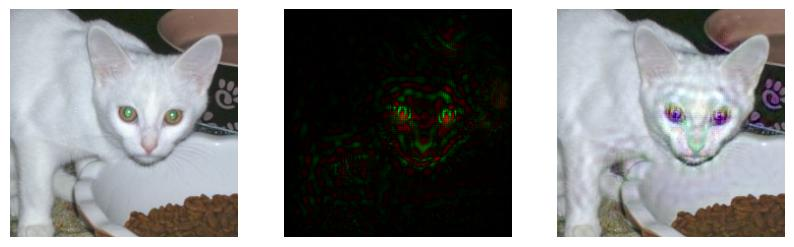
\includegraphics[width=.464\linewidth] {img/catvsdog/expl_1.jpg} &
            \hspace{-4mm}
        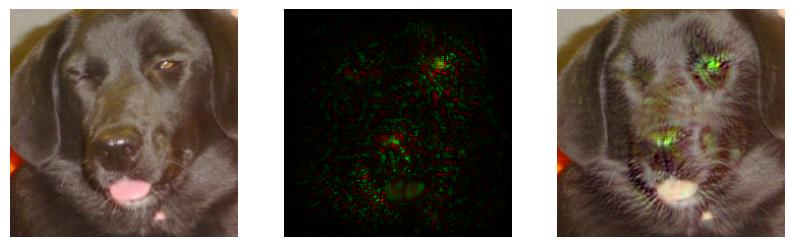
\includegraphics[width=.464\linewidth] {img/catvsdog/expl_2.jpg}\\
        & \textbf{cat $\to$ dog} & \textbf{dog $\to$ cat}\\
        % \midrule
        % \multicolumn{3}{c}{Imagenet :left cabbage butterfly to monarch one,  right great grey owl to bald eagle} \\
        \rotatebox{90}{\quad Imagenet}\hspace{-5mm} &
        
\includegraphics[width=.464\linewidth] {img/imagenet/expl_1.jpg} &
            \hspace{-4mm}
        
\includegraphics[width=.464\linewidth] {img/imagenet/expl_2.jpg} \\
        & \textbf{cabbage butterfly $\to$ monarch butterfly} & \textbf{great grey owl $\to$ bald eagle}\\
     \end{tabular}
    \caption{Samples of counterfactuals from different datasets: (left) source image , (center) gradient image, (right) counterfactual of the form $\x-t*\hat{f}(\x)\nabla_x \hat{f}(\x)$, for  $t>1$}
    \label{fig:celebA_counterfactual}
\end{figure*}
\fi

